%%%%%%%%%%%%%%%%%%%%%%%% ExtendedAbstract.tex %%%%%%%%%%%%%%%%%%%%%%%%
%                                                                    %
%  Template for the 10-page extended abstract to be submitted for    %
%  the MSc degree conferral at Instituto Superior Tecnico.           %
%                                                                    %
%  Author:                                                           %
%                                                                    %
%       Andre C. Marta                                               %
%       Area Cientifica de Mecanica Aplicada e Aeroespacial          %
%       Departamento de Engenharia Mecanica                          %
%       Instituto Superior Tecnico                                   %
%       Av. Rovisco Pais                                             %
%       1049-001 Lisboa                                              %
%       Portugal                                                     %
%       Tel: +351 21 841 9466                                        %
%                        3466 (extension)                            %
%       Email: andre.marta@ist.utl.pt                                %
%                                                                    %
%  Created:       Dec  2, 2011                                       %
%  Last Modified: Dec 27, 2011                                       %
%%%%%%%%%%%%%%%%%%%%%%%%%%%%%%%%%%%%%%%%%%%%%%%%%%%%%%%%%%%%%%%%%%%%%%
% This document uses the LaTeX class file "article.cls"              %
%%%%%%%%%%%%%%%%%%%%%%%%%%%%%%%%%%%%%%%%%%%%%%%%%%%%%%%%%%%%%%%%%%%%%%
\documentclass[10pt,a4paper,twocolumn]{article}

%%%%%%%%%%%%%%%%%%%%%%%%%%%%%%%%%%%%%%%%%%%%%%%%%%%%%%%%%%%%%%%%%%%%%%
% Document preamble
%%%%%%%%%%%%%%%%%%%%%%%%%%%%%%%%%%%%%%%%%%%%%%%%%%%%%%%%%%%%%%%%%%%%%%

%% Builds upon the graphics  package, providing a key-value interface
%% for optional arguments to the \includegraphics command that go far
%% beyone what the graphics package offers.
%% http://www.ctan.org/tex-archive/help/Catalogue/entries/graphicx.html
%% if you use PostScript figures in your article
%% use the graphics package for simple commands
%% \usepackage{graphics}
%% or use the graphicx package for more complicated commands
%% \usepackage{graphicx}
%% or use the epsfig package if you prefer to use the old commands
%% \usepackage{epsfig}
\usepackage{graphicx} % Enhanced LaTeX Graphics
% Improve double-column float handling and reduce whitespace from floats
% (Avoid extra packages that may be unavailable in the build env)
% Page geometry: tighter margins for better content fit
\usepackage[a4paper,top=15mm,bottom=20mm,left=15mm,right=15mm]{geometry}
% Slightly reduce space between columns
\setlength{\columnsep}{6mm}

% Tighter vertical spacing around floats/captions to avoid large gaps
\setlength{\textfloatsep}{8pt plus 2pt minus 2pt}
\setlength{\dbltextfloatsep}{8pt plus 2pt minus 2pt}
\setlength{\intextsep}{8pt plus 2pt minus 2pt}
\setlength{\abovecaptionskip}{3pt}
\setlength{\belowcaptionskip}{0pt}

% Encourage flexible float placement to reduce unwanted gaps
\renewcommand{\topfraction}{0.95}
\renewcommand{\bottomfraction}{0.85}
\renewcommand{\textfraction}{0.05}
\renewcommand{\floatpagefraction}{0.8}
\renewcommand{\dbltopfraction}{0.95}
\renewcommand{\dblfloatpagefraction}{0.8}

% For colored text
\usepackage{xcolor}

% For clickable URLs
\usepackage{url}

% For professional table rules (toprule, midrule, bottomrule)
\usepackage{booktabs}

% For multirow cells in tables
\usepackage{multirow}

% Multiple figures
\usepackage{subfigure} % subcaptions for subfigures
%\usepackage{subfigmat} % matrices of similar subfigures (not available on this system)

% Declaring new column types
% 'dcolumn' package defines D to be a column specifier with
% three arguments: D{<sep.tex>}{<sep.dvi>}{<decimal places>}
%                  D{<sep.tex>}{<sep.dvi>}{<left digit places>.<right digit places>}
\usepackage{dcolumn}           % decimal-aligned tabular math columns
% d takes a single argument specifying the number of decimal places, e.g., d{2}
% or the number of digits to the left and right of the seperator, e.g., d{3.2}
\newcolumntype{.}   {D{.}{.}{-1}} % column alignedd on the point separator '.'
\newcolumntype{d}[1]{D{.}{.}{#1}} % column centered on the point separator '.'
\newcolumntype{e}   {D{E}{E}{-1}} % column centered on the exponent 'E'
\newcolumntype{E}[1]{D{E}{E}{#1}} % column centered on the exponent 'E'

%% American Mathematical Society (AMS) plain Tex macros
%%
%% The amsmath package is the principal package in the AMS-LaTeX distribution
%% http://www.ctan.org/tex-archive/help/Catalogue/entries/amsmath.html
\usepackage{amsmath}
%%
%% The amsfonts package provides extended TeX fonts
%% http://www.ctan.org/tex-archive/help/Catalogue/entries/amsfonts.html
\usepackage{amsfonts}
%% The amssymb package provides various useful mathematical symbols
\usepackage{amssymb}
%%
%% The amsthm package provides extended theorem environments
%% http://www.ctan.org/tex-archive/help/Catalogue/entries/amsthm.html
\usepackage{amsthm}

%% Improves the interface for defining floating objects such as figures and tables.
%% The package also provides the H float modifier option of the obsolete here package.
%% http://www.ctan.org/tex-archive/help/Catalogue/entries/float.html
\usepackage{float}

%% Control sectional headers. 
%% http://www.ctan.org/tex-archive/help/Catalogue/entries/sectsty.html
\usepackage{sectsty}
%%
%% Redefine the font size of the 'section' and 'subsection' headings
\newcommand{\myFontSize}{\fontsize{11}{0}\selectfont}
\newcommand{\mySubFontSize}{\fontsize{10}{0}\selectfont}
\sectionfont{\myFontSize\bfseries}       % 11pt, Bold face
\subsectionfont{\mySubFontSize\bfseries} % 10pt, Bold face

%% Select alternative section titles.
%% http://www.ctan.org/tex-archive/help/Catalogue/entries/titlesec.html
\usepackage{titlesec}
%%
%% Left indent, before and after spacing
%% (The starred version kills the indentation of the paragraph following the title)
\titlespacing*{\section}{0pt}{12pt}{6pt}
\titlespacing*{\subsection}{0pt}{10pt}{4pt}

%% Section numbers with trailing dots using titlesec (secdot not available)
%% Alternative implementation using titlesec package
\titleformat{\section}{\myFontSize\bfseries}{\thesection.}{1em}{}
\titleformat{\subsection}{\mySubFontSize\bfseries}{\thesubsection.}{1em}{}

% Slightly reduce body font size to improve layout fit
\AtBeginDocument{\small}

% Margins now controlled by geometry; remove manual overrides

% New command to refer to equations as Eq.(1),Eq.(2),...
\newcommand{\eqnref}[1]{Eq.(\ref{#1})}

%%%%%%%%%%%%%%%%%%%%%%%%%%%%%%%%%%%%%%%%%%%%%%%%%%%%%%%%%%%%%%%%%%%%%%%%%%%%%%%%%%%%%%%%
% Title, authors and addresses

\title{Open-Vocabulary Semantic Segmentation of Aerial Photos}
\date{September 2025}
\author{Luis Pedro Soares Marnoto Gaspar Lopes \\ luis.marnoto.gaspar.lopes@tecnico.ulisboa.pt \\ \\ Instituto Superior T\'{e}cnico, Lisboa, Portugal}

%%%%%%%%%%%%%%%%%%%%%%%%%%%%%%%%%%%%%%%%%%%%%%%%%%%%%%%%%%%%%%%%%%%%%%%%%%%%%%%%%%%%%%%%
\begin{document}

% Begin one column section for title and abstract
%
% http://www.faqs.org/faqs/de-tex-faq/part5/
\twocolumn[
\begin{@twocolumnfalse}
\maketitle

%%%%%%%%%%%%%%%%%%%%%%%%%%%%%%%%%%%%%%%%%%%%%%%%%%%%%%%%%%%%%%%%%%%%%%
% ABSTRACT & KEYWORDS
%%%%%%%%%%%%%%%%%%%%%%%%%%%%%%%%%%%%%%%%%%%%%%%%%%%%%%%%%%%%%%%%%%%%%%
%%%%%%%%%%%%%%%%%%%%%%%%%%%%%%%%%%%%%%%%%%%%%%%%%%%%%%%%%%%%%%%%%%%%%%
%     File: ExtendedAbstract_abstr.tex                               %
%     Tex Master: ExtendedAbstract.tex                               %
%%%%%%%%%%%%%%%%%%%%%%%%%%%%%%%%%%%%%%%%%%%%%%%%%%%%%%%%%%%%%%%%%%%%%%

\begin{abstract}

\noindent{{\bf Keywords:}} 

\end{abstract}



% End one column section (begin default two columns)
\end{@twocolumnfalse}
]
%%%%%%%%%%%%%%%%%%%%%%%%%%%%%%%%%%%%%%%%%%%%%%%%%%%%%%%%%%%%%%%%%%%%%%
% INTRODUCTION
%%%%%%%%%%%%%%%%%%%%%%%%%%%%%%%%%%%%%%%%%%%%%%%%%%%%%%%%%%%%%%%%%%%%%%
%%%%%%%%%%%%%%%%%%%%%%%%%%%%%%%%%%%%%%%%%%%%%%%%%%%%%%%%%%%%%%%%%%%%%%
%     File: ExtendedAbstract_intro.tex                               %
%     Tex Master: ExtendedAbstract.tex                               %
%%%%%%%%%%%%%%%%%%%%%%%%%%%%%%%%%%%%%%%%%%%%%%%%%%%%%%%%%%%%%%%%%%%%%%

\section{Introduction}
\label{sec:intro}

Referring expression segmentation is a computer vision task in which a model receives a natural language description of a target region and must return the corresponding segmentation mask. Because the phrasing can reference any concept, the task is open-vocabulary and the target can be a single instance, a coherent group of instances, or an entire semantic category, such as "all roads in the patch" or "the vegetation strip along the river". The remote-sensing literature coined the term Referring Remote Sensing Instance Segmentation (RRSIS)~\cite{yuan2023rrsis} for the subset that limits expressions to single instances, while later datasets like NWPU-Refer~\cite{yang2024large} incorporated group-level expressions and Aerial-D extends the coverage further to include instances, groups, and full land-cover classes. When this formulation is applied to aerial photographs, although we refer to it simply as referring expression segmentation throughout this article, the problem becomes especially demanding because top-down perspectives compress object scales, spatial resolution varies across sensors, many targets occupy only a handful of pixels, and the scenes themselves contain extreme object densities. In many real deployments, analysts revisit archival aerial surveys to study how cities or coastlines evolved. To support that use case, the pipeline also models the monochrome, sepia, and grainy degradations found in historic imagery so the resulting models can handle tasks such as assessing long-term urban change.

A critical component for developing effective models for RRSIS is access to high-quality datasets containing aerial photographs, precise segmentation masks, and natural referring expressions. To address this need, this work presents Aerial-D, a large-scale referring expression segmentation dataset for aerial imagery comprising 1,522,523 expressions across 37,288 aerial image patches, compared with prior RRSIS datasets~\cite{yuan2023rrsis,liu2024rotated,yang2024large}. Figure~\ref{fig:dataset_examples} highlights how this corpus spans rural and urban scenes and objects, land-cover regions, groups of multiple objects, and entire categories while retaining unrestricted, richly worded referring expressions tailored to each target. Each sample further includes an automatically generated historic counterpart, enabling models trained on the dataset to understand black-and-white, grainy, or sepia aerial imagery alongside contemporary captures.

% Locally tighten spacing for this figure to avoid a visible gap
\begingroup
\setlength{\intextsep}{6pt}
\setlength{\abovecaptionskip}{2pt}
\setlength{\belowcaptionskip}{0pt}
\begin{figure}[H]
\centering
\includegraphics[width=\columnwidth]{./images/6samples.png}
\caption{Representative examples from Aerial-D dataset showing diverse referring expressions with corresponding aerial images and ground truth masks.}
\label{fig:dataset_examples}
\end{figure}
\endgroup


The key contributions of this work include: (1) a comprehensive toolchain that enables the production of complex referring expression datasets from instance segmentation datasets, including a rule-based pipeline, Large Language Model enhancement and distillation methods, and historic image data augmentation with dedicated filtering; (2) the construction of Aerial-D, a dataset comprising over 1.5 million expressions across 37,288 aerial image patches, created entirely through the proposed automatic pipeline; and (3) a unified model trained on Aerial-D alongside four additional datasets, applying the full toolchain—including historic transformations across all training data—to deliver referring expression segmentation over instances, groups, classes, and land cover regions while maintaining reliable performance on degraded historic imagery typical of archival aerial surveys.


%%%%%%%%%%%%%%%%%%%%%%%%%%%%%%%%%%%%%%%%%%%%%%%%%%%%%%%%%%%%%%%%%%%%%%
% RELATED WORK
%%%%%%%%%%%%%%%%%%%%%%%%%%%%%%%%%%%%%%%%%%%%%%%%%%%%%%%%%%%%%%%%%%%%%%
%%%%%%%%%%%%%%%%%%%%%%%%%%%%%%%%%%%%%%%%%%%%%%%%%%%%%%%%%%%%%%%%%%%%%%
%     File: ExtendedAbstract_backg.tex                               %
%     Tex Master: ExtendedAbstract.tex                               %
%%%%%%%%%%%%%%%%%%%%%%%%%%%%%%%%%%%%%%%%%%%%%%%%%%%%%%%%%%%%%%%%%%%%%%

\section{Related Work}
\label{sec:related}

This section examines the foundational datasets and architectural innovations that have shaped aerial image understanding, focusing on instance segmentation, land-cover analysis, referring segmentation, historical imagery, and specialized model architectures for remote sensing applications.

\subsection{Foundational Datasets}

\subsubsection{Instance and Semantic Segmentation}

The iSAID dataset~\cite{zamir2019isaid} established the foundation for instance segmentation in aerial imagery by providing 655,451 object instances across 15 categories in 2,806 high-resolution images. Building upon the DOTA dataset, iSAID addressed the unique challenges of aerial imagery including high object density, large scale variations, and arbitrary orientations. The dataset demonstrated that existing computer vision methods require specialized adaptation for aerial domains, as off-the-shelf approaches achieved suboptimal performance.

Complementing instance-level analysis, the LoveDA dataset~\cite{wang2021loveda} focused on land-cover semantic segmentation across urban and rural environments. Covering 536.15 km² with 0.3m resolution imagery, LoveDA enables domain adaptation research by addressing style differences between geographical environments, with urban scenes dominated by artificial objects and rural scenes containing natural elements.

\subsubsection{Referring Segmentation Evolution}

The transition from traditional segmentation to language-guided approaches began with RefSegRS~\cite{yuan2023rrsis}, which introduced the first referring remote sensing image segmentation dataset with 4,420 image-language-label triplets, establishing the RRSIS task and addressing challenges of small and scattered objects in remote sensing imagery.

RRSIS-D~\cite{liu2024rotated} represents the largest referring remote sensing image segmentation dataset with 17,402 image-caption-mask triplets, three times larger than its predecessors. The dataset utilized semi-automated annotation through the Segment Anything Model (SAM) for efficient dataset creation while maintaining annotation quality. RRSIS-D addresses unique challenges in aerial imagery including vast spatial scales and diverse object orientations across 20 different object categories and seven attribute dimensions, providing comprehensive evaluation capabilities for referring segmentation methods.

The NWPU-Refer dataset~\cite{yang2024large} further expanded scale with 15,003 high-resolution images containing 49,745 annotated targets across 30+ countries. This dataset emphasizes purely manual annotation processes for enhanced quality and supports single-object, multi-object, and non-object segmentation scenarios across 32 object categories.

\subsubsection{Historical Imagery Applications}

The Urban1960SatSeg dataset~\cite{hao2025urban1960satseg} addresses the critical gap in historical aerial imagery analysis by providing the first professionally annotated semantic segmentation dataset using mid-20th century declassified satellite imagery. Covering 1,240 km² of Xi'an, China, this dataset enables quantitative analysis of urban development patterns from the 1960s through novel unsupervised segmentation frameworks designed for grayscale, distorted historical imagery.

\subsection{Architectures for RRSIS}

Specialized architectures for referring remote sensing image segmentation have evolved to address the unique complexities of aerial imagery. The foundational RefSegRS work established basic approaches for combining language understanding with aerial image segmentation, while subsequent developments introduced more sophisticated solutions for overhead imagery challenges.

The Rotated Multi-Scale Interaction Network (RMSIN)~\cite{liu2024rotated} represents a significant architectural advancement specifically designed for remote sensing image complexities. RMSIN addresses the unique challenges in aerial imagery through three key technical modules: the Intra-scale Interaction Module (IIM) for fine-grained detail extraction, the Cross-scale Interaction Module (CIM) for comprehensive feature fusion across different scales, and Adaptive Rotated Convolution (ARC) for handling rotational variations common in aerial scenes. RMSIN achieved state-of-the-art performance with 3.64\% and 3.16\% mIoU improvements over the closest competitor LAVT, demonstrating the effectiveness of specialized architectural design for aerial imagery.

The RSRefSeg architecture~\cite{chen2025rsrefseg} pioneered the integration of foundation models for remote sensing by effectively combining CLIP and SAM. This 1.2 billion parameter model introduced the AttnPrompter bridge mechanism to convert textual semantic features into SAM-compatible prompts, achieving strong performance (cIoU: 77.04, gIoU: 64.65) through parameter-efficient LoRA fine-tuning.

The MRSNet framework~\cite{yang2024large} further advances multi-scale processing through specialized Intra-scale Feature Interaction Modules (IFIM) and Hierarchical Feature Interaction Modules (HFIM), contributing to the continued evolution of architectures tailored for aerial imagery understanding.



%%%%%%%%%%%%%%%%%%%%%%%%%%%%%%%%%%%%%%%%%%%%%%%%%%%%%%%%%%%%%%%%%%%%%%
% APPROACH FOR DATASET GENERATION
%%%%%%%%%%%%%%%%%%%%%%%%%%%%%%%%%%%%%%%%%%%%%%%%%%%%%%%%%%%%%%%%%%%%%%
%%%%%%%%%%%%%%%%%%%%%%%%%%%%%%%%%%%%%%%%%%%%%%%%%%%%%%%%%%%%%%%%%%%%%%
%     File: ExtendedAbstract_imple.tex                               %
%     Tex Master: ExtendedAbstract.tex                               %
%%%%%%%%%%%%%%%%%%%%%%%%%%%%%%%%%%%%%%%%%%%%%%%%%%%%%%%%%%%%%%%%%%%%%%

\section{Aerial-D Dataset Construction}
\label{sec:approach}

\subsection{Rule-Based Expression Generation}

\begin{figure*}[t]
\centering
\begin{minipage}{0.5\textwidth}
\centering
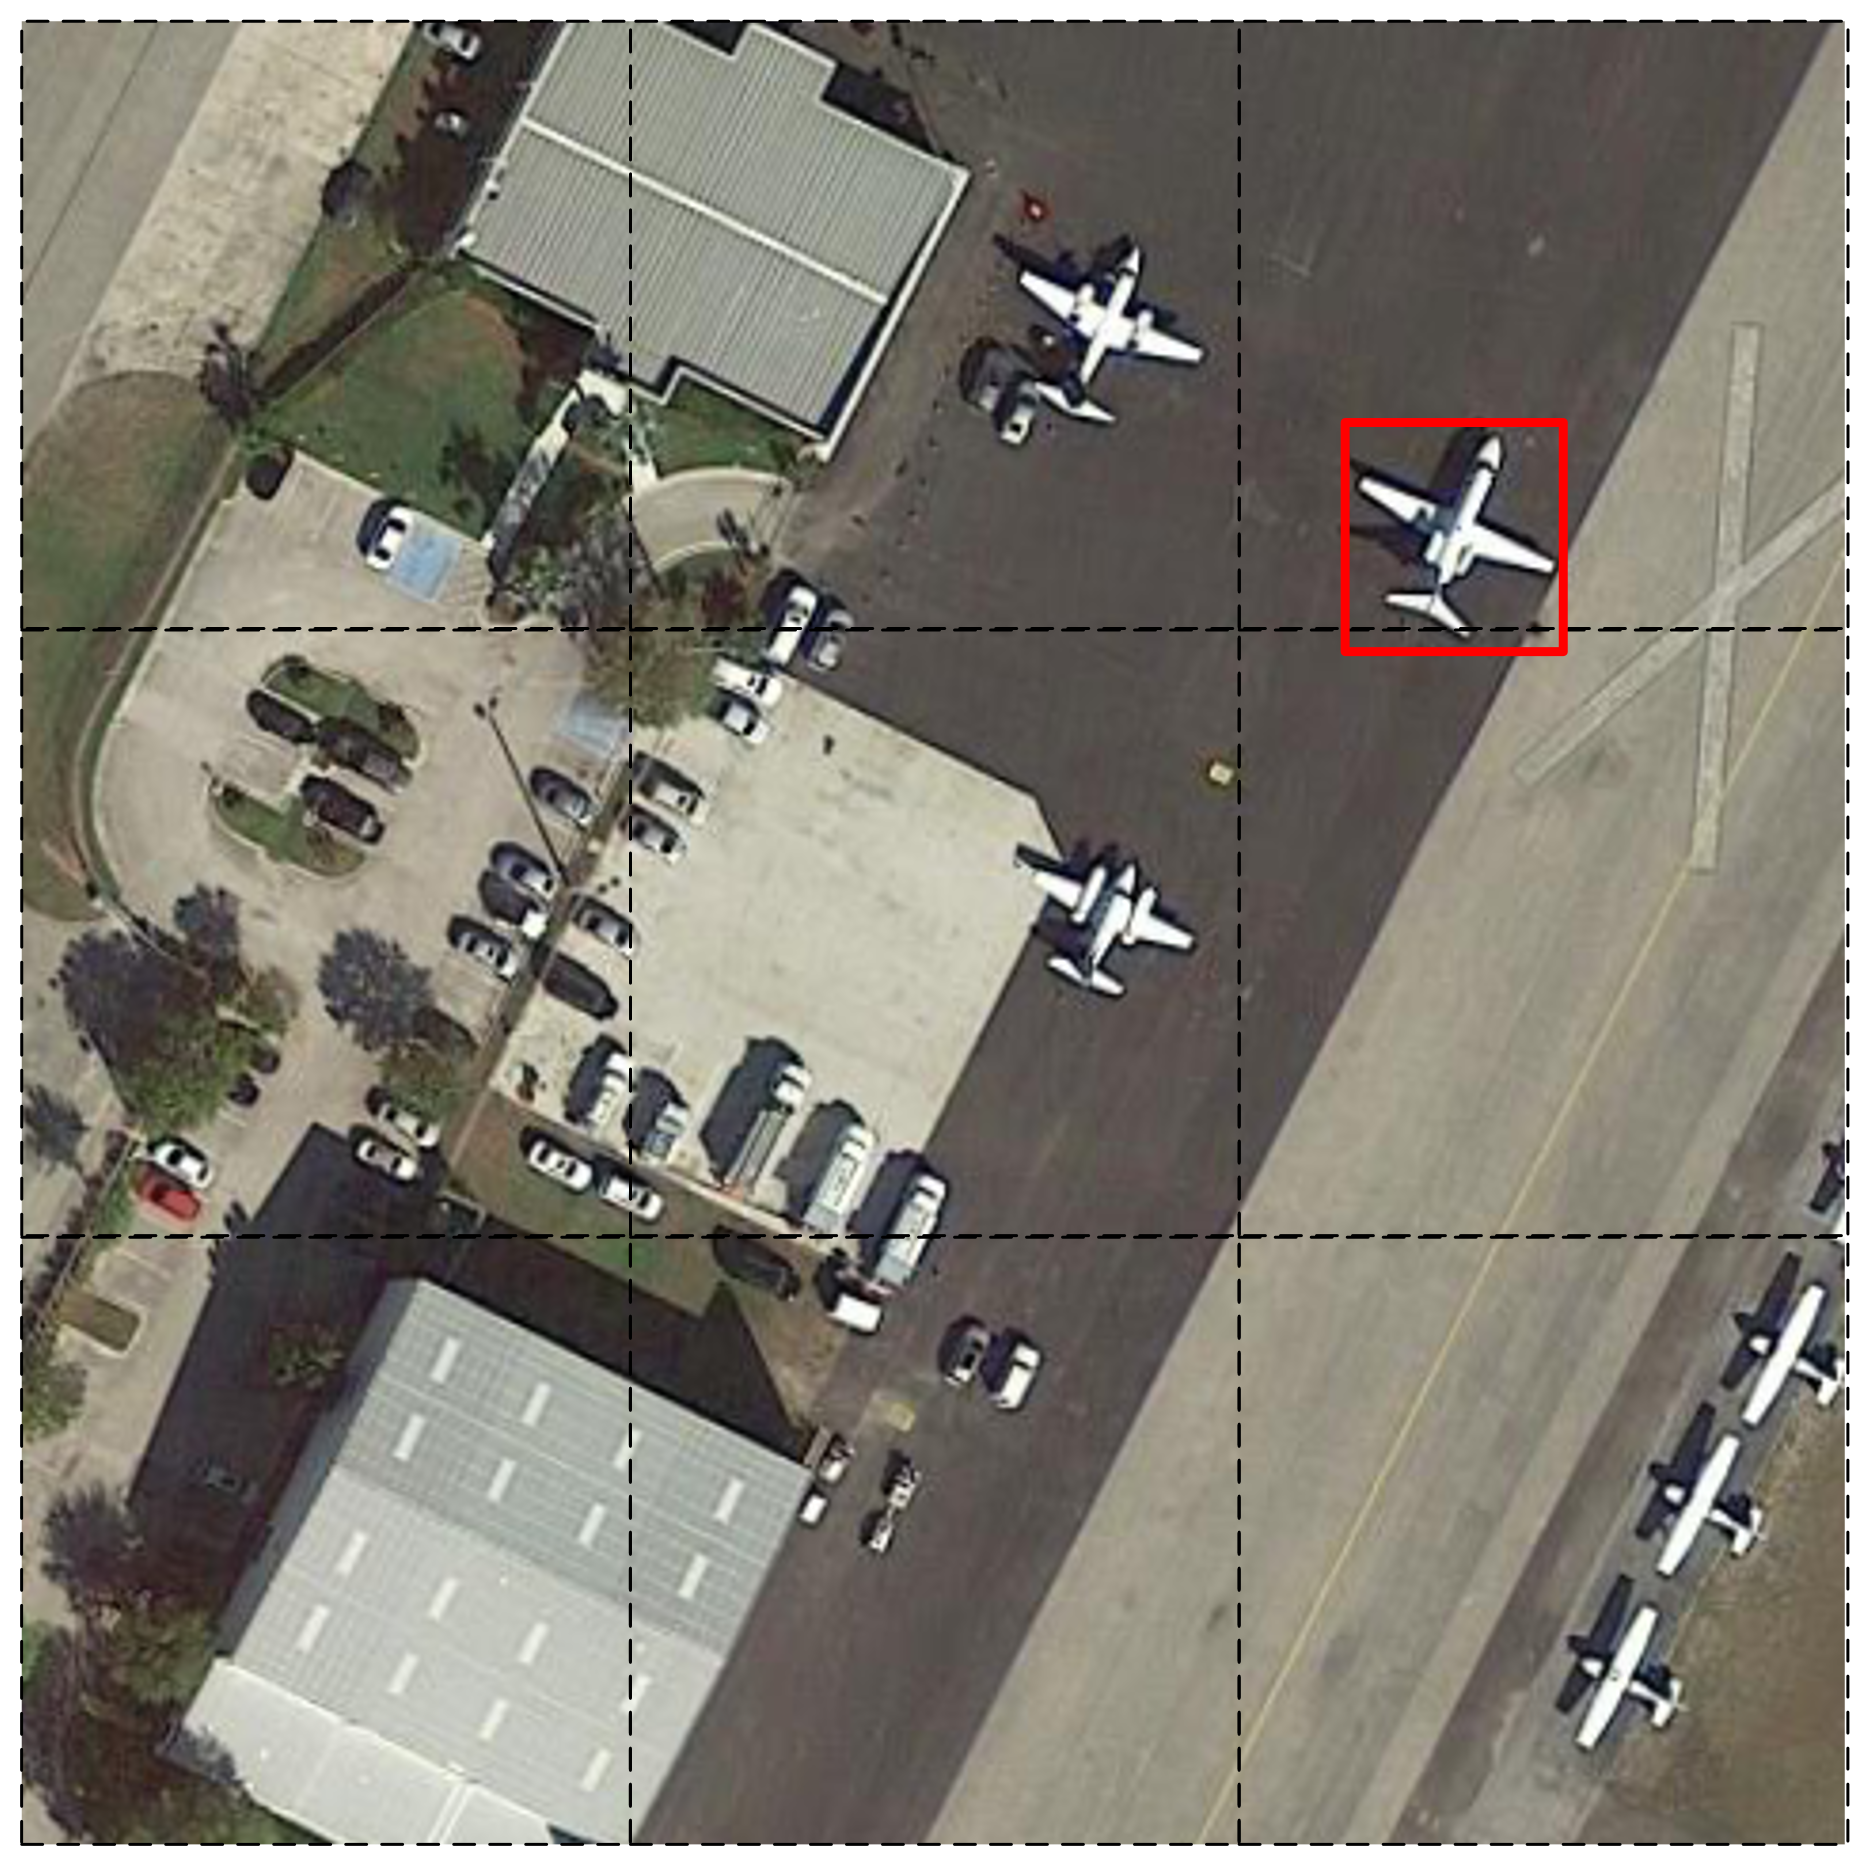
\includegraphics[width=0.7\textwidth]{./images/rule_based_generation.png}
\end{minipage}%
\begin{minipage}{0.5\textwidth}
\centering
\hspace{-1cm}
\raisebox{-0.3\height}{%
\resizebox{\textwidth}{!}{%
\footnotesize
\begin{tabular}{@{}ll@{}}
\toprule
\textbf{Rule Type} & \textbf{Example Instance} \\
\midrule
Category & "plane" \\
Grid Position & "in the top right" \\
Extreme Position & None \\
Color Classification & "light" \\
Directional Relations & "to the bottom right of a plane" \\
& "to the top right of a plane" \\
\midrule
\multicolumn{2}{l}{\textbf{Final Expressions}} \\
\multicolumn{2}{l}{"the plane in the top right"} \\
\multicolumn{2}{l}{"the light plane in the top right"} \\
\multicolumn{2}{l}{"the plane in the top right to the bottom right of a plane"} \\
\multicolumn{2}{l}{"the light plane in the top right to the bottom right of a plane"} \\
\multicolumn{2}{l}{"the plane in the top right to the top right of a plane"} \\
\multicolumn{2}{l}{"the light plane in the top right to the top right of a plane"} \\
\bottomrule
\end{tabular}%
}%
}
\end{minipage}
\caption{Example of rule generation for a single instance. The highlighted plane in the top right section demonstrates how the system assigns spatial, visual, and relational rules that will later be combined into referring expressions.}
\label{fig:rule_example}
\end{figure*}


\subsection{LLM Expression Generation}

\begin{figure*}[t]
\centering
\begin{minipage}{0.5\textwidth}
\centering
\includegraphics[width=0.7\textwidth]{./images/example_group.png}
\end{minipage}%
\begin{minipage}{0.5\textwidth}
\centering
\hspace{-1cm}
\raisebox{-0.3\height}{%
\footnotesize
\begin{tabular}{@{}p{2cm}p{5cm}@{}}
\toprule
\textbf{Expression Type} & \textbf{Example} \\
\midrule
Original & the group of 4 large vehicles in the top center \\
\midrule
Enhanced & the cluster of four big vehicles near the upper middle \\
\midrule
Unique & the four large vehicles lined up side by side just below the pale paved strip at the very top middle \\
\midrule
Unique & the set of four big vehicles parked in a single row in the upper center beside the grassy area to the right \\
\bottomrule
\end{tabular}%
}
\end{minipage}
\caption{Example of LLM enhancement process showing original aerial image with group of four large vehicles (left) and corresponding expression enhancements (right).}
\label{fig:llm_enhancement_example}
\end{figure*}


\begin{figure}[H]
\centering
\includegraphics[width=0.8\columnwidth]{./images/distillation.png}
\caption{Knowledge distillation pipeline for scalable LLM enhancement. A small sample of 500 expressions is processed through OpenAI's O3 model to generate high-quality training targets, which are then used to fine-tune Gemma3 12B via QLora. The fine-tuned model enables cost-effective local inference to enhance the full dataset of 300,000 expressions using vLLM on a single GPU.}
\label{fig:llm_distillation}
\end{figure}


%%%%%%%%%%%%%%%%%%%%%%%%%%%%%%%%%%%%%%%%%%%%%%%%%%%%%%%%%%%%%%%%%%%%%%
% EXPERIMENTS
%%%%%%%%%%%%%%%%%%%%%%%%%%%%%%%%%%%%%%%%%%%%%%%%%%%%%%%%%%%%%%%%%%%%%%
%%%%%%%%%%%%%%%%%%%%%%%%%%%%%%%%%%%%%%%%%%%%%%%%%%%%%%%%%%%%%%%%%%%%%%
%     File: ExtendedAbstract_resul.tex                               %
%     Tex Master: ExtendedAbstract.tex                               %
%%%%%%%%%%%%%%%%%%%%%%%%%%%%%%%%%%%%%%%%%%%%%%%%%%%%%%%%%%%%%%%%%%%%%%

\section{Experiments}
\label{sec:experiments}

This section presents a comprehensive experimental evaluation of Aerial-D that spans model training, cross-dataset generalization, and targeted ablations. We first describe the model architecture and training setup, then report cross-dataset results on established aerial referring expression segmentation datasets. Beyond aggregate performance, we also include: (i) ablation of expression enhancement strategies; (ii) ablation of historic-filter training; and (iii) qualitative comparison across language models (o3, base Gemma3, and our distilled Gemma3-Aerial model), coupled with a cost analysis of these alternatives.

\subsection{Model Architecture}
\label{subsec:model_architecture}

In selecting the architecture for our experiments, we prioritized a model that can interpret natural-language descriptions while producing pixel-accurate masks in aerial scenes. Generic segmentation systems rarely meet both requirements under the domain shift of remote sensing, where objects are small, repetitive, and densely arranged. We therefore adopt RSRefSeg as our backbone for referring expression segmentation: it pairs a strong language–image encoder (SigLIP2) with a state-of-the-art mask decoder (SAM), enabling robust semantic grounding alongside precise mask generation. As in the original RSRefSeg training, the model is fine‑tuned via LoRA adapters; we retain this recipe when adapting to the remote‑sensing domain. This choice is further supported by the strong performance reported for RSRefSeg on RRSIS-D\cite{liu2024rotated}, providing a proven baseline for aerial referring expression segmentation and reducing risk in our evaluation.

Concretely, we implement the RSRefSeg architecture\cite{chen2025rsrefseg} in PyTorch, as illustrated in Figure~\ref{fig:rsrefseg_arch}. The design couples SigLIP2\cite{siglip2} for vision–language encoding with SAM\cite{sam} for mask generation. Following the original authors, training uses LoRA (Low‑Rank Adaptation)\cite{lora} adapters inserted into the SAM image encoder and into SigLIP2’s vision and text encoders, while preserving the strong pretraining of these backbones. In practice, adapters are placed on the query and value projection layers in the vision encoders and on the query, key, value, and output projection layers in the text encoder.

\subsection{Experimental Setup}
\label{subsec:experimental_setup}

Our training configuration uses a batch size of 4 with gradient accumulation steps of 2, achieving an effective batch size of 8 samples. The model employs \texttt{SigLIP2-SO400M} for vision–language encoding and \texttt{SAM-ViT-Large} for mask generation when training the combined model. Consistent with the RSRefSeg training strategy, we employ LoRA with rank \(r=32\) for parameter‑efficient adaptation. Training uses AdamW optimizer\cite{adamw} with initial learning rate of 1e-4, weight decay of 0.01, and polynomial learning rate decay with power factor 0.9. Mixed-precision computation and gradient clipping with maximum norm of 1.0 ensure training stability. Inputs are prepared per backbone: images are resized to 384×384 for SigLIP2 and to 1024×1024 for SAM. The historic filters described in Section~\ref{subsec:historic_filters} are incorporated during data preparation for the four non‑historic datasets (Aerial‑D, RRSIS‑D, NWPU‑Refer, RefSegRS): for each dataset, we randomly select 20\% of training images and replace them with a single filtered copy, sampling one of the three filters uniformly for each selected image.

In order to prevent Aerial-D from overwhelming the combined training mix, we limit its contribution to the \emph{Unique Expressions Only} split identified in the ablation below. This choice keeps the total number of Aerial-D samples closer to the scale of the four public datasets—each of which contributes only tens of thousands of expressions—while still exposing the model to the richer cues that the unique-only subset provides. We train the resulting combined model on Aerial-D (unique-only), RRSIS-D\cite{liu2024rotated}, NWPU-Refer\cite{yang2024large}, RefSegRS\cite{yuan2023rrsis}, and Urban1960SatSeg\cite{hao2025urban1960satseg}, and evaluate on their validation splits (Aerial-D uses the \emph{combined-all} validation set). To probe robustness to historical degradations, we additionally evaluate historic-filtered counterparts obtained by converting 100\% of validation images for the four non-historic datasets (Aerial-D, RRSIS-D, NWPU-Refer, RefSegRS) using the three filters from Section~\ref{subsec:historic_filters}. We report these results under the "Hist." columns.

\subsection{Evaluation Results}
\label{subsec:evaluation_results}

Tables~\ref{tab:aeriald_variants} and \ref{tab:combined_training_results} report validation results for the combined model trained jointly on all datasets. Both tables focus on mean IoU and overall IoU for the original validation splits alongside their historic-filtered counterparts, highlighting aggregate overlap rather than thresholded pass rates.

Table~\ref{tab:aeriald_variants} isolates Aerial-D and breaks the evaluation down by supervision type. The instance-only view concentrates on explicit object targets, the semantic configuration captures land-cover regions, and the combined variant merges both sources to reflect the full dataset mixture. Rows list the two checkpoints we trained—RSRefSeg-b and the larger RSRefSeg-l—with the latter awaiting full evaluation, hence the placeholder entries.

Across the external benchmarks in Table~\ref{tab:combined_training_results}, the RSRefSeg-b checkpoint maintains strong performance. On RRSIS-D we measure 61.70\% mIoU and 73.44\% oIoU, with the historic split retaining \textcolor{blue}{58.35\%} and \textcolor{blue}{71.73\%}. NWPU-Refer records 37.89\% mIoU and 51.34\% oIoU, dropping to \textcolor{blue}{31.52\%} and \textcolor{blue}{46.17\%} under filters. RefSegRS lands at 40.10\% mIoU and 45.05\% oIoU, tapering to \textcolor{blue}{32.79\%} and \textcolor{blue}{36.74\%} on its historic counterpart. Urban1960SatSeg, already composed of archival imagery, posts 69.35\% mIoU and 87.27\% oIoU. These scores match or surpass previously reported baselines across the public datasets while defining reference values for Aerial-D. The RSRefSeg-l checkpoint is undergoing validation; its row is included for completeness with placeholders until evaluation concludes.

The combined model therefore achieves comparable results to previously reported baselines on every public benchmark while simultaneously establishing reference numbers for Aerial-D. The narrow gap between original and historic evaluations shows that the augmentation strategy meaningfully improves robustness without sacrificing accuracy on contemporary imagery, and the pending RSRefSeg-l run will extend this comparison once metrics are available.

\begin{table*}[t]
\centering
\caption{Aerial-D supervision variants evaluated on the validation split (historic scores in \textcolor{blue}{blue}; ``--'' denotes metrics that are not yet available).}
\label{tab:aeriald_variants}
\resizebox{\textwidth}{!}{%
\begin{tabular}{@{}l|cc|cc|cc@{}}
\toprule
\multirow{2}{*}{\textbf{Model}} & \multicolumn{2}{c|}{\textbf{Instance Targets}} & \multicolumn{2}{c|}{\textbf{Semantic Regions}} & \multicolumn{2}{c}{\textbf{Instance + Semantic}} \\
\cmidrule(lr){2-3} \cmidrule(lr){4-5} \cmidrule(lr){6-7}
 & \textbf{mIoU} & \textbf{oIoU} & \textbf{mIoU} & \textbf{oIoU} & \textbf{mIoU} & \textbf{oIoU} \\
\midrule
\textbf{RSRefSeg-b (ours)} & 49.78\% / \textcolor{blue}{46.82\%} & 63.44\% / \textcolor{blue}{61.12\%} & -- & -- & 49.78\% / \textcolor{blue}{46.82\%} & 63.44\% / \textcolor{blue}{61.12\%} \\
\textbf{RSRefSeg-l (ours)} & -- & -- & -- & -- & -- & -- \\
\bottomrule
\end{tabular}%
}
\end{table*}

\begin{table*}[t]
\centering
\caption{Cross-dataset validation results for RSRefSeg variants (ours) and published baselines (historic scores in \textcolor{blue}{blue}; ``--'' indicates metrics not reported in the cited work).}
\label{tab:combined_training_results}
\resizebox{\textwidth}{!}{%
\begin{tabular}{@{}l|cc|cc|cc|cc@{}}
\toprule
\multirow{2}{*}{\textbf{Model}} & \multicolumn{2}{c|}{\textbf{RefSegRS}} & \multicolumn{2}{c|}{\textbf{RRSIS-D}} & \multicolumn{2}{c|}{\textbf{NWPU-Refer}} & \multicolumn{2}{c}{\textbf{Urban1960SatSeg}} \\
\cmidrule(lr){2-3} \cmidrule(lr){4-5} \cmidrule(lr){6-7} \cmidrule(lr){8-9}
 & \textbf{mIoU} & \textbf{oIoU} & \textbf{mIoU} & \textbf{oIoU} & \textbf{mIoU} & \textbf{oIoU} & \textbf{mIoU} & \textbf{oIoU} \\
\midrule
\textbf{RSRefSeg-b (ours)} & 40.10\% / \textcolor{blue}{32.79\%} & 45.05\% / \textcolor{blue}{36.74\%} & 61.70\% / \textcolor{blue}{58.35\%} & 73.44\% / \textcolor{blue}{71.73\%} & 37.89\% / \textcolor{blue}{31.52\%} & 51.34\% / \textcolor{blue}{46.17\%} & 69.35\% & 87.27\% \\
\textbf{RSRefSeg-l (ours)} & -- & -- & -- & -- & -- & -- & -- & -- \\
\midrule
LAVT\cite{liu2024rotated} & -- & -- & 61.46\% & 77.59\% & -- & -- & -- & -- \\
RMSIN\cite{liu2024rotated,yang2024large,chen2025rsrefseg} & 59.96\% & 76.81\% & 65.10\% & 78.27\% & 41.75\% & 62.66\% & -- & -- \\
RSRefSeg-b\cite{chen2025rsrefseg} & -- & -- & 63.68\% & 76.05\% & -- & -- & -- & -- \\
RSRefSeg-l\cite{chen2025rsrefseg} & -- & -- & -- & -- & -- & -- & -- & -- \\
MRSNet\cite{yang2024large} & -- & -- & -- & -- & 44.86\% & 63.59\% & -- & -- \\
\bottomrule
\end{tabular}%
}
\end{table*}

\subsection{Expression Enhancement Ablation}
\label{subsec:ablation_studies}

In order to quantify how much the enhanced expressions improve segmentation outcomes, we revisit Aerial-D with a controlled experiment. The combined model in Section~\ref{subsec:evaluation_results} blends rule-based descriptions with LLM rewrites, which makes it difficult to isolate the specific contribution of each expression type when comparing against the original, simpler phrasing. We therefore retrain RSRefSeg on Aerial-D with a lighter setup—SAM-ViT-Base replaces SAM-ViT-Large to accelerate the runs, and the LoRA rank is lowered to \(r=16\) while keeping all other optimizer settings, learning schedules, and preprocessing identical to Section~\ref{subsec:experimental_setup}. This configuration keeps the focus on the language differences rather than architectural changes.

Using this setup, we train four separate models, each exposed to a distinct slice of Aerial-D: (i) \emph{Rule-based Only} retains the original deterministic descriptions produced by the rule system; (ii) \emph{Enhanced Only} relies on LLM rewrites that diversify the wording while preserving the target; (iii) \emph{Unique Expressions Only} selects LLM augmentations that inject alternative visual cues; and (iv) \emph{Combined All} unites the three sources. Figure~\ref{fig:llm_enhancement_example} illustrates how the enhanced variants expand the phrasing beyond the rule-based baseline. We evaluate the resulting checkpoints on four validation sets without additional tuning: Aerial-D (using the \emph{combined-all} validation split) and three external datasets—RefSegRS, RRSIS-D, and NWPU-Refer—to observe how each expression type supports generalization beyond the training distribution.

Table~\ref{tab:ablation_expression_types} summarizes the results and explicitly reports both the number of \emph{Samples} and \emph{Epochs} used per configuration. Looking across datasets, several consistent patterns emerge. On Aerial-D, the \emph{Combined All} configuration achieves the best accuracy, which is expected given that the validation distribution matches that training mixture. For the three external datasets, different subsets yield the strongest generalization: on RRSIS-D, varying the language (\emph{Enhanced Only}) helps most; on NWPU-Refer, emphasizing varied visual cues (\emph{Unique Expressions Only}) is most beneficial; and on RefSegRS, a combination of both types provides the best results. These outcomes highlight the breadth of ways to phrase referring expressions and show that leveraging LLMs to introduce targeted variety improves cross-dataset generalization.

In order to keep early stopping responsive to each subset, we monitor validation loss across the four runs and halt training as soon as it begins to rebound. Because the \emph{Combined All} subset is roughly three times larger than the others, its validation loss ticks upward immediately after the second epoch, so we stop that run at two epochs. The three smaller subsets continue improving through the fourth epoch before showing the same rise, allowing four full passes over their data. This schedule means that the language-variation and unique-only models actually process fewer total samples than the combined run, yet they surpass it on RRSIS-D and NWPU-Refer. The outcome reveals that curated expression subsets can be more sample efficient than the full mixture, which is why the combined model in Section~\ref{subsec:evaluation_results} draws on the unique-only split of Aerial-D. Beyond sample efficiency, constraining Aerial-D to that subset keeps the cross-dataset mix from being dominated by a single corpus whose expression pool would otherwise reach into the millions.

% Ablation expression types table with explicit epochs and samples
\begin{table*}[t]
\centering
\caption{Expression Enhancement Ablation Across Four Datasets}
\label{tab:ablation_expression_types}
\resizebox{\textwidth}{!}{%
\begin{tabular}{@{}lcc|cc|cc|cc|cc@{}}
\toprule
\multirow{2}{*}{\textbf{Training Configuration}} & \multirow{2}{*}{\textbf{Samples}} & \multirow{2}{*}{\textbf{Epochs}} & \multicolumn{2}{c|}{\textbf{Aerial-D}} & \multicolumn{2}{c|}{\textbf{RefSegRS}} & \multicolumn{2}{c|}{\textbf{RRSIS-D}} & \multicolumn{2}{c}{\textbf{NWPU-Refer}} \\
\cmidrule(lr){4-5} \cmidrule(lr){6-7} \cmidrule(lr){8-9} \cmidrule(lr){10-11}
 & & & % \textbf{Pass@0.7} & 
\textbf{mIoU} & \textbf{oIoU} & % \textbf{Pass@0.7} & 
\textbf{mIoU} & \textbf{oIoU} & % \textbf{Pass@0.7} & 
\textbf{mIoU} & \textbf{oIoU} & % \textbf{Pass@0.7} & 
\textbf{mIoU} & \textbf{oIoU} \\
\midrule
Rule-based Only & 371K & 4 & % 26.81\% & 
34.57\% & 39.31\% & % 2.55\% & 
3.73\% & 0.55\% & % 29.89\% & 
34.22\% & 36.46\% & % 13.62\% & 
16.78\% & 13.70\% \\
Enhanced Only & 364K & 4 & % 36.39\% & 
46.45\% & 56.99\% & % \textbf{3.02\%} & 
5.75\% & 4.99\% & % \textbf{35.63\%} & 
\textbf{41.63\%} & \textbf{42.48\%} & % \textbf{16.90\%} & 
21.89\% & 16.68\% \\
Unique Expressions Only & 382K & 4 & % 35.75\% & 
46.54\% & 63.02\% & % 2.55\% & 
18.32\% & 8.37\% & % 20.86\% & 
31.78\% & 33.73\% & % 15.91\% & 
\textbf{24.68\%} & \textbf{29.22\%} \\
Combined All & 1,118K & 2 & % \textbf{39.54\%} & 
\textbf{49.33\%} & \textbf{64.30\%} & % 1.86\% & 
\textbf{18.80\%} & \textbf{8.58\%} & % 23.39\% & 
34.07\% & 34.80\% & % 15.91\% & 
24.57\% & 28.27\% \\
\bottomrule
\end{tabular}%
}
\end{table*}

\subsection{Distillation Ablation: Gemma3 vs. o3 Model Comparison}
\label{subsec:distillation_ablation}

This ablation measures how the generator choice inside the LLM enhancement stage affects expression quality and overall cost. We evaluate three options for producing the enhanced expressions: OpenAI’s o3, the off‑the‑shelf Gemma3‑12B, and the distilled Gemma3-Aerial model described in Section~\ref{subsec:llm_expression_generation} (see Figure~\ref{fig:llm_distillation}).

All three models are prompted and decoded in the same way so that differences stem from the generator rather than the interface. The base Gemma3 baseline frequently hallucinates objects that are not present, which undermines segmentation training. Distillation sharply reduces those errors, producing grounded descriptions that resemble the o3 outputs while remaining accessible on local hardware.

Table~\ref{tab:cost_comparison} quantifies the practical impact. Running o3 across \(\sim\)300{,}000 targets would cost roughly \$6.2K, whereas the distilled Gemma3 produces comparable guidance for about \$26—roughly 238× cheaper because inference runs locally instead of via a commercial API. Figure~\ref{fig:distillation_comparison} illustrates why the student is worth training: the base Gemma3 hallucinates a second baseball diamond that does not exist, while the distilled variant stays aligned with the image and mirrors the grounded detail that o3 provides.

% Cost comparison table
\begin{table}[t]
\centering
\caption{Cost Analysis: Gemma3 vs. o3 Model for Large-Scale Annotation\protect\footnotemark}
\label{tab:cost_comparison}
\resizebox{\columnwidth}{!}{%
\begin{tabular}{@{}lcc@{}}
\toprule
\textbf{Model} & \textbf{Cost per request} & \textbf{Cost for 300K requests} \\
\midrule
o3 Model & \$0.020728 & \$6,218.32 \\
Distilled Gemma3 & \$0.000087 & \$26.01 \\
\midrule
\textbf{Savings} & \textbf{238× cheaper} & \textbf{\$6,192.31 (99.6\%)} \\
\bottomrule
\end{tabular}%
}
\end{table}
\footnotetext{Cost calculations based on API pricing — o3: \$2.00 per million input tokens, \$8.00 per million output tokens (OpenAI API platform); Gemma3-12B: \$0.035 per million input tokens, \$0.141 per million output tokens (OpenRouter inference provider). Average tokens per request: o3 (1,670.8 input, 2,173.3 output), Gemma3 (1,330.0 input, 284.7 output). Calculations based on 15 sample requests.}

\begin{figure*}[t]
\centering
\begin{minipage}{0.5\textwidth}
\centering
\includegraphics[width=0.65\textwidth]{./images/3llm.png}
\end{minipage}%
\begin{minipage}{0.5\textwidth}
\centering
\hspace{-1cm}
\raisebox{-0.3\height}{%
\footnotesize
\begin{tabular}{@{}p{2cm}p{5cm}@{}}
\toprule
\textbf{Expression Type} & \textbf{Example} \\
\midrule
Original & the orange baseball diamond in the top left \\
\midrule
o3 Enhanced & the orange baseball diamond with the light pole near home plate in the upper left \\
\midrule
Gemma3 Base & the bright orange baseball diamond to the left of another similar baseball diamond in the top left \\
\midrule
Gemma3-Aerial-12B & the orange baseball field with a chainlink fence surrounded by grass to the north and trees to the west \\
\bottomrule
\end{tabular}%
}
\end{minipage}
\caption{Qualitative comparison between o3, vanilla Gemma3 base model, and our fine-tuned Gemma3-Aerial-12B model on aerial imagery. The table shows how each model enhances the original rule-based expression using an identical prompt and decoding setup, demonstrating the progression from basic rule-based descriptions through increasingly capable LLM enhancements.}
\label{fig:distillation_comparison}
\end{figure*}


\subsection{Historic Filter Ablation Study}
\label{subsec:historic_ablation}

In order to understand how much the historic-image filters described in Section~\ref{subsec:historic_filters} contribute to robustness, we repeat the combined training without injecting those filters. Models that only encounter clean, contemporary imagery typically falter when historic photographs suddenly introduce monochrome toning, contrast loss, or sepia casts. We therefore run an ablation that removes the filters from the training mix and compares the resulting model against the full recipe.

Table~\ref{tab:historic_ablation_results} consolidates this experiment together with a second variant that also withholds Urban1960SatSeg from the training mix, removing the only corpus of genuinely historic imagery. Without that anchor the model still inches upward on clean validation data, yet the historic counterparts absorb far steeper losses: Aerial-D's historic mIoU slides from 46.82\% in the baseline to 38.12\%, RRSIS-D drops from 58.35\% to 52.41\%, and RefSegRS falls to 24.11\%, erasing over eight points of overlap. The impact is even more pronounced on the historic Urban imagery—the model that never observes Urban1960SatSeg during training records only 53.02\% mIoU and 70.11\% oIoU on that dataset, forfeiting roughly sixteen and seventeen percentage points respectively. These outcomes demonstrate that synthetic filters mitigate modest domain shifts, but authentic historic supervision is essential once color and contrast cues deviate from contemporary aerial photography.

Each entry in Table~\ref{tab:historic_ablation_results} reports the clean mIoU and oIoU together with the corresponding historic-filtered score (shown in \textcolor{blue}{blue}); percentage-point deltas relative to the full-training baseline are included in parentheses. Because the filter-free model encounters degradations for the first time during evaluation, the clean columns climb a few points while the historic counterparts respond unevenly: RRSIS-D and NWPU-Refer remain resilient, whereas RefSegRS still sheds about five points of mIoU. Removing Urban1960SatSeg further amplifies those losses across every historic split.
% Historic filter ablation table
\begin{table*}[t]
\centering
\caption{Historic-filter ablations. Each row lists Orig. / \textcolor{blue}{Hist.} scores with percentage-point deltas relative to Table~\ref{tab:combined_training_results}; the second block also removes Urban1960SatSeg supervision.}
\label{tab:historic_ablation_results}
\renewcommand{\arraystretch}{1.1}
\begin{tabular}{@{}llcccc@{}}
\toprule
\textbf{Training Setup} & \textbf{Dataset} & \textbf{mIoU (Orig.)} & \textbf{mIoU (Hist.)} & \textbf{oIoU (Orig.)} & \textbf{oIoU (Hist.)} \\
\midrule
\multirow{5}{*}{No Filters (All datasets)} & Aerial-D & 49.21\% (\textcolor{red}{-0.57}) & \textcolor{blue}{43.57\%} (\textcolor{red}{-3.25}) & 62.88\% (\textcolor{red}{-0.56}) & \textcolor{blue}{58.14\%} (\textcolor{red}{-2.98}) \\
 & RRSIS-D & 64.36\% (\textcolor{darkgreen}{+2.66}) & \textcolor{blue}{59.02\%} (\textcolor{darkgreen}{+0.67}) & 75.59\% (\textcolor{darkgreen}{+2.15}) & \textcolor{blue}{72.50\%} (\textcolor{darkgreen}{+0.77}) \\
 & NWPU-Refer & 41.06\% (\textcolor{darkgreen}{+3.17}) & \textcolor{blue}{33.42\%} (\textcolor{darkgreen}{+1.90}) & 58.35\% (\textcolor{darkgreen}{+7.01}) & \textcolor{blue}{53.04\%} (\textcolor{darkgreen}{+6.87}) \\
 & RefSegRS & 41.31\% (\textcolor{darkgreen}{+1.21}) & \textcolor{blue}{27.73\%} (\textcolor{red}{-5.06}) & 50.30\% (\textcolor{darkgreen}{+5.25}) & \textcolor{blue}{32.21\%} (\textcolor{red}{-4.53}) \\
 & Urban1960SatSeg & 69.81\% (\textcolor{darkgreen}{+0.46}) & -- & 87.80\% (\textcolor{darkgreen}{+0.53}) & -- \\
\midrule
\multirow{5}{*}{No Urban + No Filters} & Aerial-D & 48.12\% (\textcolor{red}{-1.66}) & \textcolor{blue}{38.12\%} (\textcolor{red}{-8.70}) & 61.07\% (\textcolor{red}{-2.37}) & \textcolor{blue}{52.91\%} (\textcolor{red}{-8.21}) \\
 & RRSIS-D & 63.58\% (\textcolor{darkgreen}{+1.88}) & \textcolor{blue}{52.41\%} (\textcolor{red}{-5.94}) & 74.92\% (\textcolor{darkgreen}{+1.48}) & \textcolor{blue}{64.38\%} (\textcolor{red}{-7.35}) \\
 & NWPU-Refer & 40.33\% (\textcolor{darkgreen}{+2.44}) & \textcolor{blue}{28.76\%} (\textcolor{red}{-2.76}) & 55.62\% (\textcolor{darkgreen}{+4.28}) & \textcolor{blue}{39.05\%} (\textcolor{red}{-7.12}) \\
 & RefSegRS & 41.25\% (\textcolor{darkgreen}{+1.15}) & \textcolor{blue}{24.11\%} (\textcolor{red}{-8.68}) & 49.88\% (\textcolor{darkgreen}{+4.83}) & \textcolor{blue}{28.45\%} (\textcolor{red}{-8.29}) \\
 & Urban1960SatSeg & 53.02\% (\textcolor{red}{-16.33}) & -- & 70.11\% (\textcolor{red}{-17.16}) & -- \\
\bottomrule
\end{tabular}
\renewcommand{\arraystretch}{1}
\end{table*}

Values in parentheses denote percentage-point change relative to the baseline combined model in Table~\ref{tab:combined_training_results}; \textcolor{blue}{blue} marks historic-filtered validation scores.

%%%%%%%%%%%%%%%%%%%%%%%%%%%%%%%%%%%%%%%%%%%%%%%%%%%%%%%%%%%%%%%%%%%%%%
% CONCLUSION AND FUTURE WORK
%%%%%%%%%%%%%%%%%%%%%%%%%%%%%%%%%%%%%%%%%%%%%%%%%%%%%%%%%%%%%%%%%%%%%%
%%%%%%%%%%%%%%%%%%%%%%%%%%%%%%%%%%%%%%%%%%%%%%%%%%%%%%%%%%%%%%%%%%%%%%
%     File: ExtendedAbstract_concl.tex                               %
%     Tex Master: ExtendedAbstract.tex                               %
%%%%%%%%%%%%%%%%%%%%%%%%%%%%%%%%%%%%%%%%%%%%%%%%%%%%%%%%%%%%%%%%%%%%%%

\section{Conclusion and Future Work}
\label{sec:conclusion}



%%%%%%%%%%%%%%%%%%%%%%%%%%%%%%%%%%%%%%%%%%%%%%%%%%%%%%%%%%%%%%%%%%%%%%
% REFERENCES
%%%%%%%%%%%%%%%%%%%%%%%%%%%%%%%%%%%%%%%%%%%%%%%%%%%%%%%%%%%%%%%%%%%%%%

% Produces the bibliography section when processed by BibTeX
%
% Bibliography style
% > entries ordered alphabetically
%\bibliographystyle{plain}
% > unsorted with entries appearing in the order in which the citations appear.
%\bibliographystyle{unsrt}
% > entries ordered alphabetically, with first names and names of journals and months abbreviated
\bibliographystyle{abbrv}
% > entries ordered alphabetically, with reference markers based on authors' initials and publication year
%\bibliographystyle{alpha}

% External bibliography database file in the BibTeX format (ExtendedAbstract_ref_db.bib)
\bibliography{ExtendedAbstract_ref_db}

%%%%%%%%%%%%%%%%%%%%%%%%%%%%%%%%%%%%%%%%%%%%%%%%%%%%%%%%%%%%%%%%%%%%%%
\end{document}
%%%%%%%%%%%%%%%%%%%%%%%%%%%%%%%%%%%%%%%%%%%%%%%%%%%%%%%%%%%%%%%%%%%%%%
